\chapter{Output files}
In general writing to disk is slow on even the most modern of computers with an SSD.  The seek speed of mechanical disks has increased little of their history.  Thus often writing the output data to the hard disk is the most time consuming part of any simulation.  By default gpvdm writes all output files to disk this is so the new user can get a feel for what output gpvdm can provide.  However to speed up simulations you should limit how much data is written to disk. The simulation editor windows (steady state,time domain etc..) offer options to decide how much data you want to dump to disk. This is shown in figure \ref{fig:jveditorwindow} 

\begin{figure}[H]
\centering
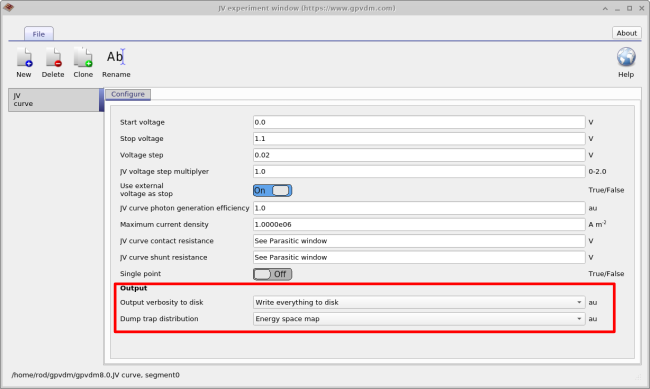
\includegraphics[width=\textwidth]{./images/jv_editor_window.png}[H]
\caption{Selecting which output files are written to disk.}
\label{fig:jveditorwindow}
\end{figure}

The option "Output verbosity to disk" can be toggled between "None" and "write everything to disk".  When "None" is selected nothing is outputted to disk at all - even simulation results are not written.  When "write everything to disk" is selected the simulation dumps everything to disk, so JV curves and all internal variables of the solver are written to disk so that the user can examine how carrier densities, fermi-levels, potentials etc.. change during the course of the simulation (see section \ref{sec:snapshots}). The second option below "Output verbosity to disk" called "dump trap distribution" will write out the distribution of traps in energy and position space.  See section \ref{sec:trapmap}.


\section{Snapshots directory - dir}
\label{sec:snapshots}
The snapshots directory (see figure \ref{fig:fileviewer}) allows the user to plot all internal solver parameters.  For example figure \ref{fig:snapshots} where the snapshots tool is being used to plot the conduction band, valance band and quasi Fermi-levels as a function of voltage.  The slider can be used to view different voltages.

\begin{figure}[H]
\centering
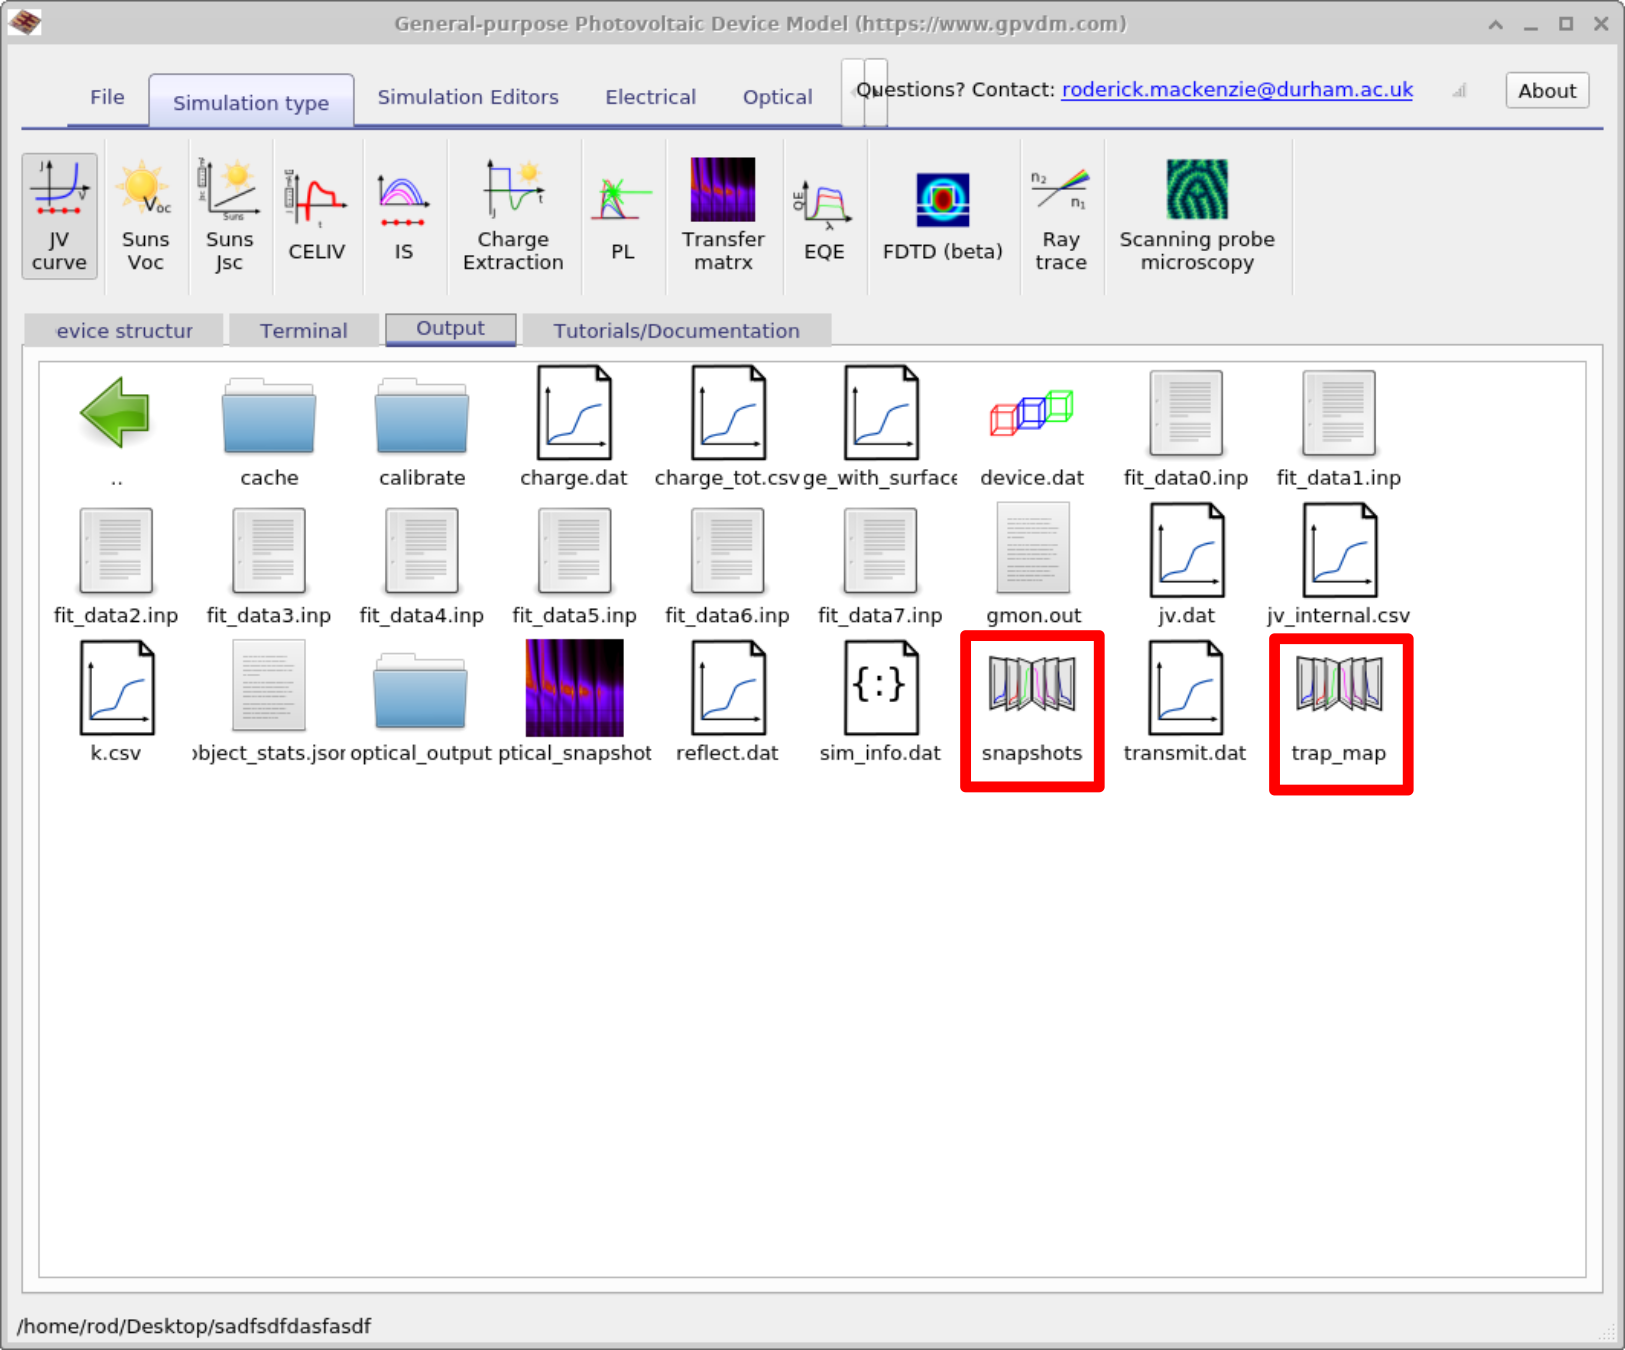
\includegraphics[width=\textwidth,height=0.7\textwidth]{./images/snapshots.png}
\caption{The file viewer showing the snapshots and trap map directory}
\label{fig:fileviewer}
\end{figure}

\begin{figure}[H]
\centering
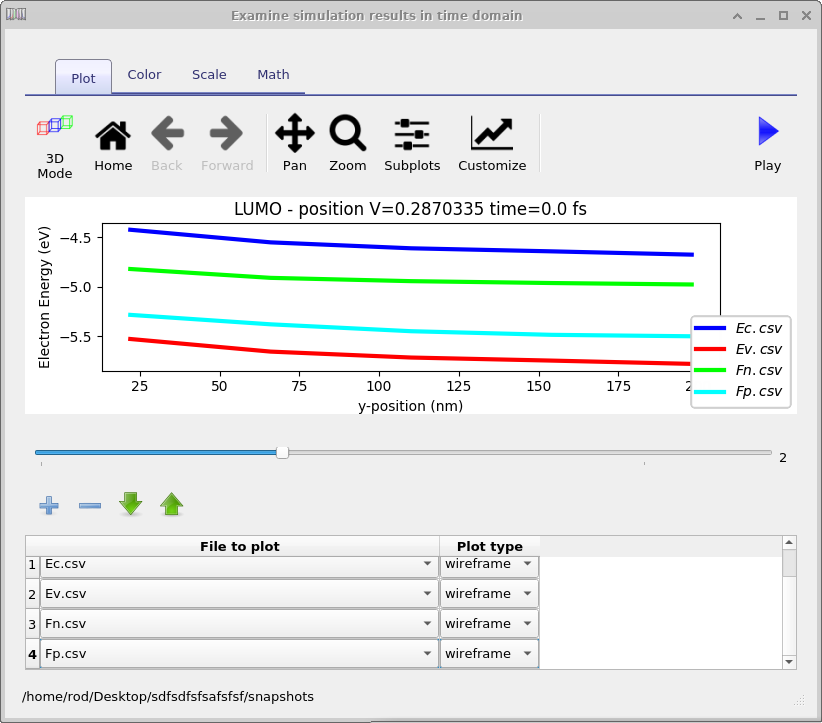
\includegraphics[width=\textwidth,height=0.7\textwidth]{./images/snapshot_viewer.png}
\caption{Using the snapshots tool to view the conduction band, valance band and quasi Fermi-levels}
\label{fig:snapshots}
\end{figure}

\section{Trap\_map directory - dir}
The trap map directory contains the distribution and density of carriers in the traps as a function of position and energetic depth. An example is given in figure \ref{fig:trapmap}
\label{sec:trapmap}


\begin{figure}[H]
\centering
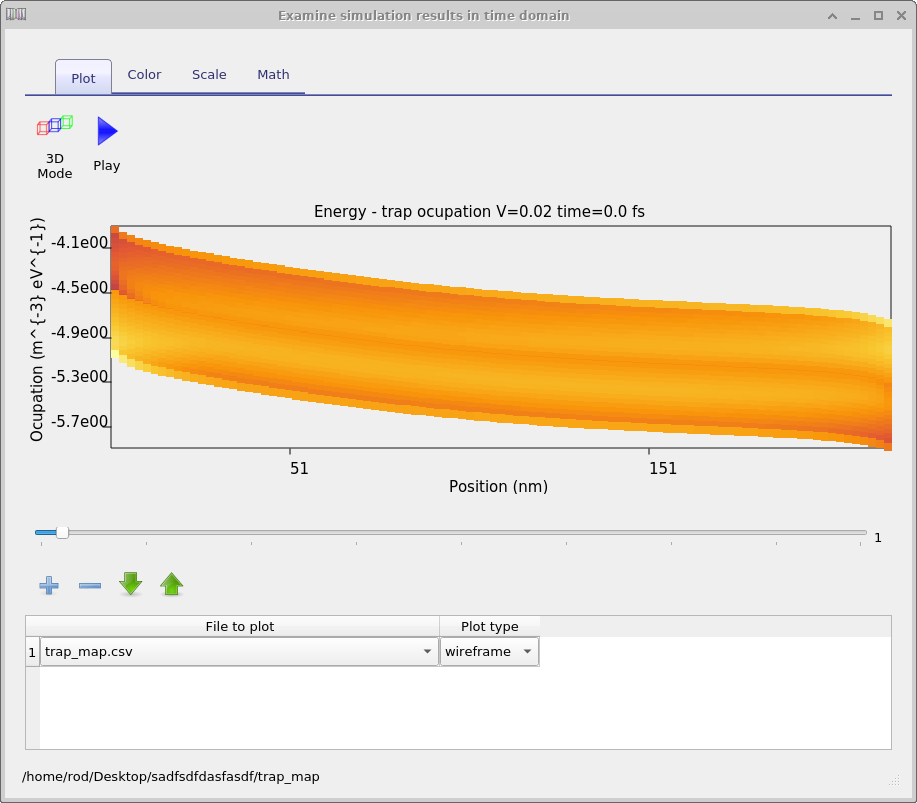
\includegraphics[width=\textwidth,height=0.7\textwidth]{./images/trapmap.png}
\caption{Plotting the position and energy dependence of carriers using the trap map tool}
\label{fig:trapmap}
\end{figure}

\section{Optical snapshots - dir}
\label{sec:snapshotsoptical}
Contains results of the optical simulations.

\section{Cache - dir}
\label{sec:cache}
Getting a computer to do math is on the whole a slow thing to do. It's much faster to precalculate results then store the answers in a look up table.  This can speed up calculations significantly.  The cahce dir stores the results of such precalculations, you can delete if you want it gpvdm will just remake it when it runs.

\section{Equilibrium directory}
Before the solver starts any simulation it solves the device equations in the dark with 0V applied bias.  The result of this calculation are placed in this directory.  The practical reason for doing this is that Newton's method only works if you give it a reasonable starting guess for any given problem.  Thus to start the solver, we guess the carrier densities at 0V in the dark, we then use Newton's method to calculate the exact carrier density profiles at 0V in the dark (results are stored in the equilibrium directory), then from this point we can work our way to other solutions say at +1V in the light.\cite{0953-8984-25-21-215301}

\section{sim\_info.dat}
\label{sec:siminfo}
This is a json file containging all key simulation metrics such as $J_{sc}$, $V_{oc}$, and example sim\_info.dat file is given below:


\subsection{Steady state electrical simulation}
\label{sec:siminfo}
In steady state electrical simulations such as performing a JV scan the sim\_info.dat outputs the following parameters.

\begin{landscape}
\begin{center}
\begin{tabular}{ |c|c|c|c| c| c|} 
\hline
Symbol & JSON token & Meaning & Units & Equ. & Ref \\
\hline
FF 				& ff 			& Fill factor										&au			&&\\
PCE 			& pce 			& PCE& percent										&			&\\
$P_{max}$ 		& $P\_{max}$ 	& Power at Pmax										&			&&\\
$V_{oc}$ 		& $V\_{oc}$ 		& $V_{oc}$ 										&			&&\\
$voc_{R}$ 		& $voc\_{R}$ 	& Recombination rate at $P_{max}$ 					&			& &\\
$jv_{voc}$  	& $jv\_{voc}$  	& 													&			&&\\
$jv_{pmax}$ 	& $jv\_{pmax}$ 	& 													&			&&\\
$voc_{nt}$ 		& $voc\_{nt}$ 	& Trapped electron carrier densiyt at $V_oc$		&			&&\\
$voc_{pt}$ 		& $voc\_{pt}$ 	& Trapped hole carrier density at $V_oc$			&			&&\\
$voc_{nf}$ 		& $voc\_{nf}$ 	& Free electron carrier densiyt at $V_oc$			&			&&\\
$voc_{pf}$ 		& $voc\_{pf}$ 	& Free hole carrier density at $V_oc$				&			&&\\
$J_{sc}$   		& $J\_{sc}$   	& $J_{sc}$											&$Am^{-2}$ 	& &\\
$jv_{jsc}$ 		& $jv\_{jsc}$ 	& Average charge density at $J_{sc}$				&$m^{-3}$ 	& &\\
$jv_{vbi}$ 		& $jv\_{vbi}$ 	& Built in voltage									& V			&&\\
$jv_{gen}$ 		& $jv\_{gen}$ 	& Average generation rate							&			&&\\
$voc_{np}$ 		& $voc\_{np}$ 	& 													&			&&\\
$j_{pmax}$ 		& $j\_{pmax}$ 	& Current at $P_{max}$								&$Am^{-2}$ 	& &\\
$v_{pmax}$ 		& $v\_{pmax}$ 	& Voltage at $P_{max}$    							&V			&  &\\
\hline
\end{tabular}
\end{center}

%Tau
\begin{center}
\begin{tabular}{ |c|c|c|c| c| c|} 
\hline
Symbol & JSON token & Meaning & Units & Equ. & Ref \\
\hline

%Mobility
$\mu_{jsc}$ 				& $mu\_{jsc}$ 				& Avg. mobility at $J_{sc}$				&$m^{2} V^{-1} s^{-1}$ 	&&\\
$\mu^{geom}_{jsc}$ 			& $mu\_geom\_jsc$ 			& Geom. avg. mobility @ $J_{sc}$		&$m^{2} V^{-1} s^{-1}$ 	&&\\
$\mu^{geom\_micro}_{jsc}$ 	& $mu\_geom\_micro\_jsc$ 	& Geom. avg. mobility @ $J_{sc}$		&$m^{2} V^{-1} s^{-1}$ 	&&\\


$\mu_{voc}$ 				& $mu\_{voc}$ 				& Average mobility @ $V_{oc}$			& $m^{2} V^{-1} s^{-1}$ &&\\
$\mu^{geom}_{voc}$ 			& $mu\_geom\_voc$ 			& Geom. avg. mobility @ $V_{oc}$		& $m^{2} V^{-1} s^{-1}$ &$\sqrt{\langle\mu_e\rangle \langle\mu_h\rangle}$&\\
$\mu^{geom\_avg}_{voc}$ 	& $mu\_geom\_micro\_voc$ 	& Geom. avg. mobility @ $V_{oc}$		& $m^{2} V^{-1} s^{-1}$ &$\langle\sqrt{mu_e \mu_h}\rangle$&\\

$\mu^e_{pmax}$ 				& $mu\_e\_{pmax}$ 			& Avg. electron mobility @ $P_{max}$	&$m^{2} V^{-1} s^{-1}$ 	&&\\
$\mu^h_{pmax}$ 				& $mu\_h\_{pmax}$ 			& Avg. hole mobility @ $P_{max}$ 		&$m^{2} V^{-1} s^{-1}$ 	&&\\
$\mu^{geom}_{pmax}$ 		& $mu\_geom\_pmax$ 			& Geom. avg. mobility @ $P_{max}$ 		&$m^{2} V^{-1} s^{-1}$ 	&$\sqrt{\langle\mu_e\rangle \langle\mu_h\rangle}$&\\
$\mu^{geom\_micro}_{pmax}$ 	& $mu\_geom\_micro\_pmax$ 	& Geom. avg. mobility @ $P_{max}$ 		&$m^{2} V^{-1} s^{-1}$ 	&$\langle\sqrt{mu_e \mu_h}\rangle$&\\
$\mu^{pmax}$ 				& $mu\_{pmax}$ 				& Avg. mobility @ $P_{max}$				&$m^{2} V^{-1} s^{-1}$ 	&&\\
\hline
\end{tabular}

\end{center}

%Tau
\begin{center}
\begin{tabular}{ |c|c|c|c| c| c|} 
\hline
Symbol & JSON token & Meaning & Units & Equ. & Ref \\
\hline


$\tau_{voc}$ 	& $tau\_{voc}$ 	&	Recom. time at $V_{oc}$	 			& s 		&	$R=(n-n0)/\tau$  & \cite{doi:10.1021/jp073056p}\\
$\tau_{pmax}$ 	& $tau\_{pmax}$ &	Recom. time at $P_{max}$				&s 			&	$R=(n-n0)/\tau$  & \cite{doi:10.1021/jp073056p}\\
$\tau_{voc}^{all}$ 	& $tau\_all\_{voc}$ 	&	Recomb. time at $V_{oc}$	& s 		&	$R=(n)/\tau$  & \cite{doi:10.1021/jp073056p}\\
$\tau_{pmax}^{all}$ 	& $tau\_all\_{pmax}$ &	Recomb. time at $P_{max}$	&s 			&	$R=(n)/\tau$  & \cite{doi:10.1021/jp073056p}\\
\hline

%Ivan's stuff
$theta_{srh}$ 	&$theta\_{srh}$ & $\theta_{SRH}$ Collection coefficient at $P_{max}$ y & au &&p.100 5.2a\cite{Summon-FETCH-bonn_catalog_45326403},\cite{PhysRevApplied.6.024001}\\
$theta_{srh}$ 	&$theta\_{srh}$ & $\theta_{SRH}$ Collection coefficient at $P_{max}$ & au &&p.100 5.2a\cite{Summon-FETCH-bonn_catalog_45326403},\cite{PhysRevApplied.6.024001}\\


\hline
\end{tabular}

\end{center}

\end{landscape}

\subsection{Optical simulation}

\begin{center}
\begin{tabular}{ |c|c|c| c|} 
\hline
JSON token & Meaning & Units & Ref \\
\hline
$J_{photo}$ & Photo current density $Am^{-2}$& &\\
$I_{photo}$ & Photo current $A$& &\\


\hline
\end{tabular}
\end{center}


\section{File formats}
Almost all input and output files associated with gpvdm are human readable, meaning that they are straight up text files.  All output files can be directly plotted in gnuplot/excel as can the input files.  Output files are currently called .dat, but they are simply text files. All configuration files are in json format so can be edit directly or by using the python json library.

\subsection{.dat files}
This type of file is a straight text file which can be imported into excel or any other plotting program. It contains two columns of data x and y. There is also a preamble in the file containing information such as units etc..  Gpvdm is moving from .dat files to .csv files.

\subsection{.csv files}
This is a straight csv file as you would expect which can be imported into any text editor.  The first line of the file is a json string containing information such as units etc.  You can ignore this. The second line of the file describes the x/y data in a human readable form then the rest of the file contains the data.

\subsection{Binary .csv files - files which are not human readable}
In some cases it is not practical to dump text files. Examples are when dealing with 3D structures.  In this case gpvdm will dump the same json header as used in the csv file but then dump a series of C floats representing the data.

